\documentclass[serif]{beamer}\usepackage[]{graphicx}\usepackage[]{color}
%% maxwidth is the original width if it is less than linewidth
%% otherwise use linewidth (to make sure the graphics do not exceed the margin)
\makeatletter
\def\maxwidth{ %
  \ifdim\Gin@nat@width>\linewidth
    \linewidth
  \else
    \Gin@nat@width
  \fi
}
\makeatother

\definecolor{fgcolor}{rgb}{0.345, 0.345, 0.345}
\newcommand{\hlnum}[1]{\textcolor[rgb]{0.686,0.059,0.569}{#1}}%
\newcommand{\hlstr}[1]{\textcolor[rgb]{0.192,0.494,0.8}{#1}}%
\newcommand{\hlcom}[1]{\textcolor[rgb]{0.678,0.584,0.686}{\textit{#1}}}%
\newcommand{\hlopt}[1]{\textcolor[rgb]{0,0,0}{#1}}%
\newcommand{\hlstd}[1]{\textcolor[rgb]{0.345,0.345,0.345}{#1}}%
\newcommand{\hlkwa}[1]{\textcolor[rgb]{0.161,0.373,0.58}{\textbf{#1}}}%
\newcommand{\hlkwb}[1]{\textcolor[rgb]{0.69,0.353,0.396}{#1}}%
\newcommand{\hlkwc}[1]{\textcolor[rgb]{0.333,0.667,0.333}{#1}}%
\newcommand{\hlkwd}[1]{\textcolor[rgb]{0.737,0.353,0.396}{\textbf{#1}}}%

\usepackage{framed}
\makeatletter
\newenvironment{kframe}{%
 \def\at@end@of@kframe{}%
 \ifinner\ifhmode%
  \def\at@end@of@kframe{\end{minipage}}%
  \begin{minipage}{\columnwidth}%
 \fi\fi%
 \def\FrameCommand##1{\hskip\@totalleftmargin \hskip-\fboxsep
 \colorbox{shadecolor}{##1}\hskip-\fboxsep
     % There is no \\@totalrightmargin, so:
     \hskip-\linewidth \hskip-\@totalleftmargin \hskip\columnwidth}%
 \MakeFramed {\advance\hsize-\width
   \@totalleftmargin\z@ \linewidth\hsize
   \@setminipage}}%
 {\par\unskip\endMakeFramed%
 \at@end@of@kframe}
\makeatother

\definecolor{shadecolor}{rgb}{.97, .97, .97}
\definecolor{messagecolor}{rgb}{0, 0, 0}
\definecolor{warningcolor}{rgb}{1, 0, 1}
\definecolor{errorcolor}{rgb}{1, 0, 0}
\newenvironment{knitrout}{}{} % an empty environment to be redefined in TeX

\usepackage{alltt}
\usetheme{Boadilla}
\usepackage{graphicx}
\usepackage[final]{animate}
\usepackage{breqn}
\usepackage{xcolor}
\usepackage{booktabs}
\usepackage{tikz}
\usetikzlibrary{decorations.pathreplacing}
\usetikzlibrary{shapes,arrows,positioning,shadows}
\usepackage{subfig}
\usepackage{pgf}

% change format of enumerated lists
\setbeamertemplate{enumerate items}[default]

\setbeamertemplate{navigation symbols}{}

%tikz objects
\tikzstyle{decision} = [diamond, draw, text width=6em, text badly centered, inner sep=2pt, top color=white, bottom color=zissou3]
\tikzstyle{block} = [rectangle, draw, text width=10em, text centered, rounded corners, minimum height=3em, minimum width=8em, top color = white, bottom color=zissou3]
\tikzstyle{declare} = [rectangle, draw, text width=10em, text centered, minimum height=3em, minimum width=8em, top color = white, bottom color=zissou3]

% knitr setup


% dependent data


% custom colors
\definecolor{zissou1}{HTML}{3B9AB2}\definecolor{zissou2}{HTML}{78B7C5}\definecolor{zissou3}{HTML}{EBCC2A}\definecolor{zissou4}{HTML}{E1AF00}\definecolor{zissou5}{HTML}{F21A00}

% my custom ggplot theme


% figure used on title page


\setbeamercolor{title}{fg=zissou1} % main title
\setbeamercolor{frametitle}{fg=zissou3, bg=zissou2} % frame titles
\setbeamercolor{structure}{fg=zissou5} % bottom banner
\setbeamercolor{normal text}{fg=zissou1}
\usebackgroundtemplate{
\includegraphics[height=\paperheight,width=\paperwidth]{fig/back_tmp.pdf}}
\IfFileExists{upquote.sty}{\usepackage{upquote}}{}
\begin{document}

\title[WRTDS in Tidal Waters]{\textbf{Adaptation of a Weighted Regression Approach to Evaluate Water Quality Trends in an Estuary}\vspace{-0.15in}}
\author[M. Beck]{Marcus W. Beck\inst{1} \and James D. Hagy III\inst{2}}

\institute[ORISE, EPA]{\inst{1} ORISE post-doc, USEPA National Health and Environmental Effects Research Laboratory, Gulf Ecology Division, \href{mailto:beck.marcus@epa.gov}{beck.marcus@epa.gov} \and \inst{2} USEPA National Health and Environmental Effects Research Laboratory, Gulf Ecology Division, \href{mailto:hagy.jim@epa.gov}{hagy.jim@epa.gov}}

\date{Nov. 9, 2015}

\titlegraphic{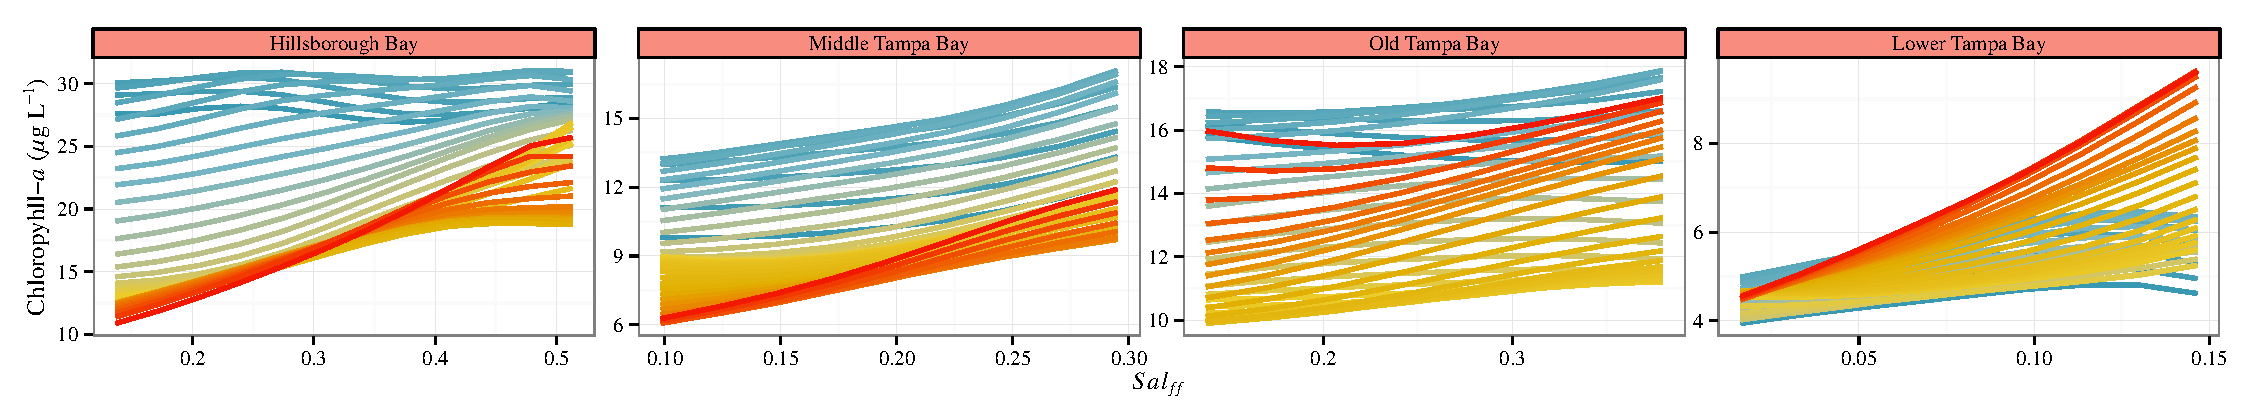
\includegraphics[width=0.9\linewidth]{fig/title_plonoleg.pdf}}

%%%%%%
\begin{frame}
\titlepage
\end{frame}

%%%%%%
\begin{frame}
\small
Beck, M.W., Hagy III, J.D. 2015. Adaptation of a weighted regression approach to evaluate water quality trends in an estuary. Environmental Modelling and Assessment. 20(6):637-655. \href{http://dx.doi.org/10.1007/s10666-015-9452-8}{doi: 10.1007/s10666-015-9452-8} \\~\\

\includegraphics[width = \textwidth]{fig/emapaper.png} 
\end{frame}

%%%%%%
\begin{frame}{\textbf{The eutrophication paradigm}}{\textbf{Research and management in coastal waters}}
\begin{quote}
Eutrophication (noun) - an \alert{increase} in the rate of supply of \alert{organic matter} to an ecosystem\\~\\
\vspace{0.05in}
\hfill -- \cite{Nixon95}
\end{quote}
\begin{center}
\scalebox{1}{
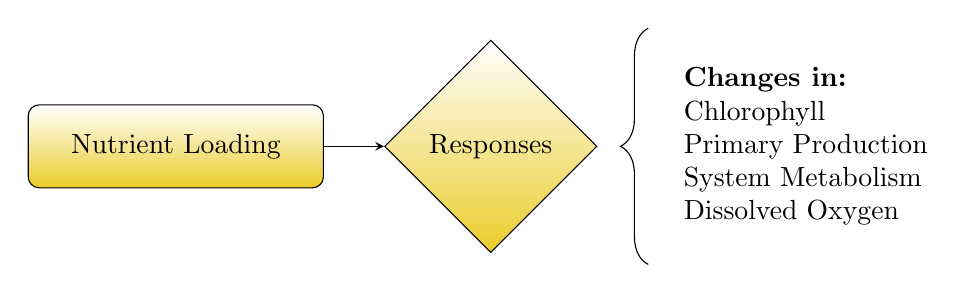
\begin{tikzpicture}[node distance = 4cm, auto, >=stealth]
  \node[block] (a) {Nutrient Loading};
	\node[decision] (b)  [right of=a] {Responses};
 	\draw[->] (a) -- (b);
  \draw[decorate,decoration={brace,amplitude=10pt}] [right of=b] (2,-1.5) -- (2,1.5);
  \node[draw,align=left,draw=none] [right of=b] {\textbf{Changes in:}\\ Chlorophyll\\ Primary Production\\ System Metabolism\\ Dissolved Oxygen};
\end{tikzpicture}}
\end{center}
\vspace{-0.5cm}\hspace*{15pt}\scalebox{0.7}{\hbox{\tiny Adapted from \cite{Cloern01}}}\\~\\
\end{frame}

% ts example


%%%%%%
\begin{frame}{\textbf{The eutrophication paradigm}}{\textbf{Research and management in coastal waters}}
Increasing availability of records describing \alert{long-term changes} \\~\\
Observed data can provide a means to an end, potentially \alert{high power} with large sample size \\~\\
Can we \alert{develop} and \alert{apply} tools that leverage the descriptive capabilities of these large datasets? \\~\\
Can we \alert{link descriptions} to \alert{causal events} to inform management or understanding?
\begin{figure}
\centerline{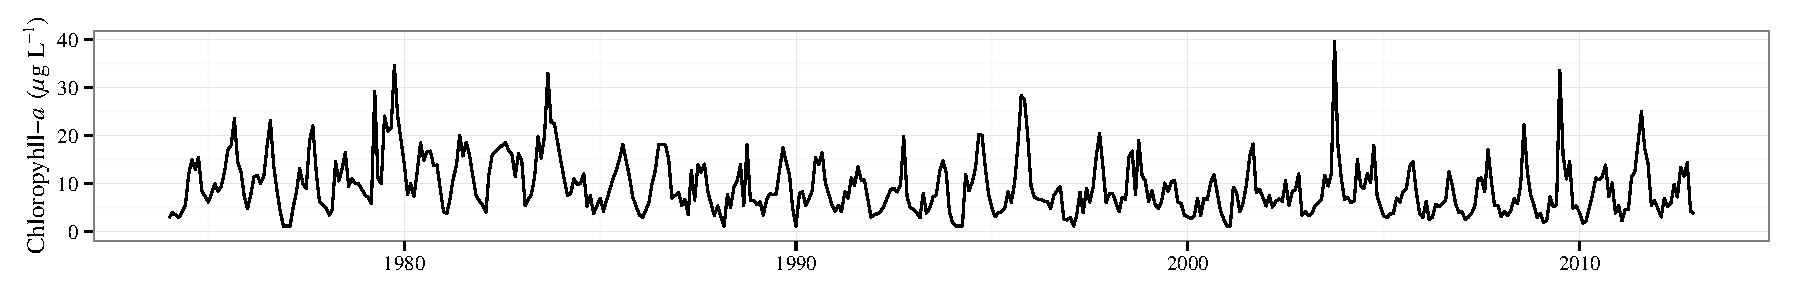
\includegraphics[width = \textwidth]{fig/ts_ex.pdf}}
\end{figure}
\end{frame}

% tampa bay map, w/ inset


%%%%%%
\begin{frame}{\textbf{Tampa Bay}}{\textbf{Understanding chlorophyll response to eutrophication}}
\begin{columns}
\begin{column}{0.5\textwidth}
\begin{itemize}
\item Four bay segments\\~\\
\item Monthly wq data at 50 stations from 1974 to present \\~\\
\item Longitudinal profile of nutrient load and salinity \\~\\
\end{itemize}
\vspace{0cm}\hspace*{15pt}\scalebox{0.7}{\hbox{\tiny Data from \cite{TBEP11}}}
\end{column}
\begin{column}{0.5\textwidth}
\centerline{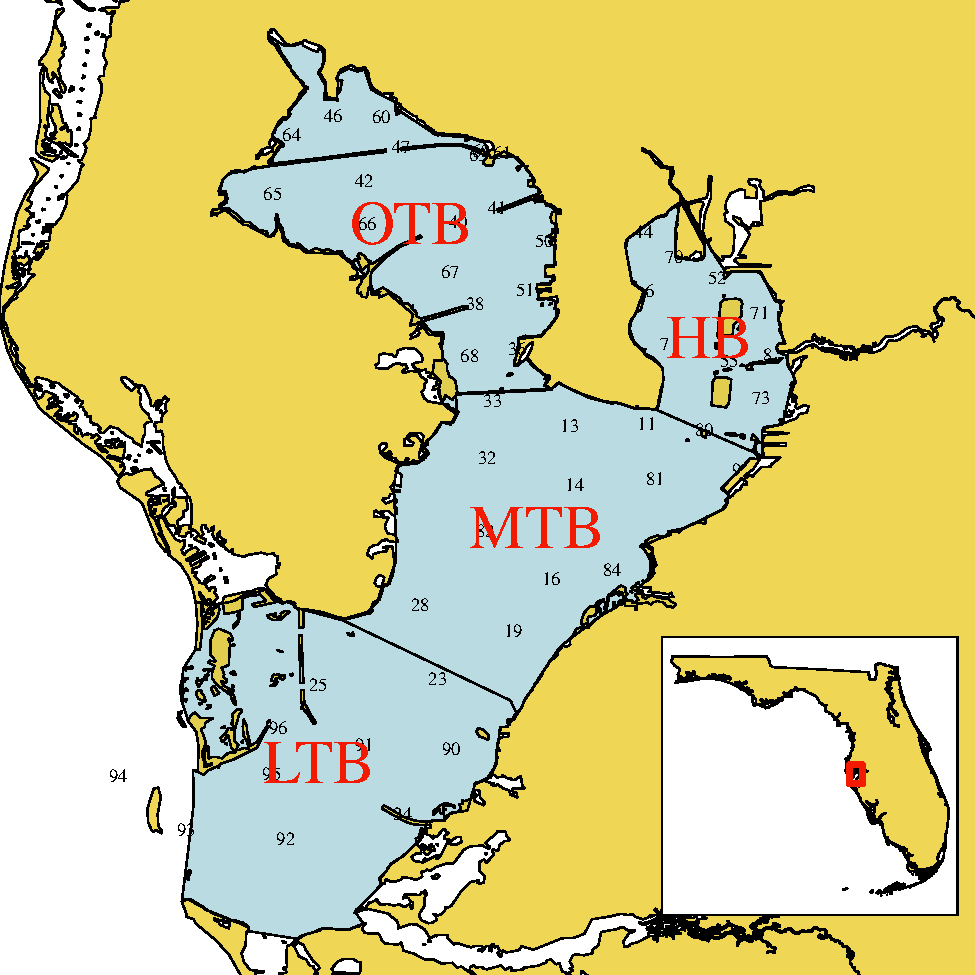
\includegraphics[width = \textwidth]{fig/tb_map.pdf}}
\end{column}
\end{columns}
\end{frame}

%%%%%%
\begin{frame}{\textbf{Tampa Bay}}{\textbf{Understanding chlorophyll response to eutrophication}}
\begin{figure}[!ht]


{\centering 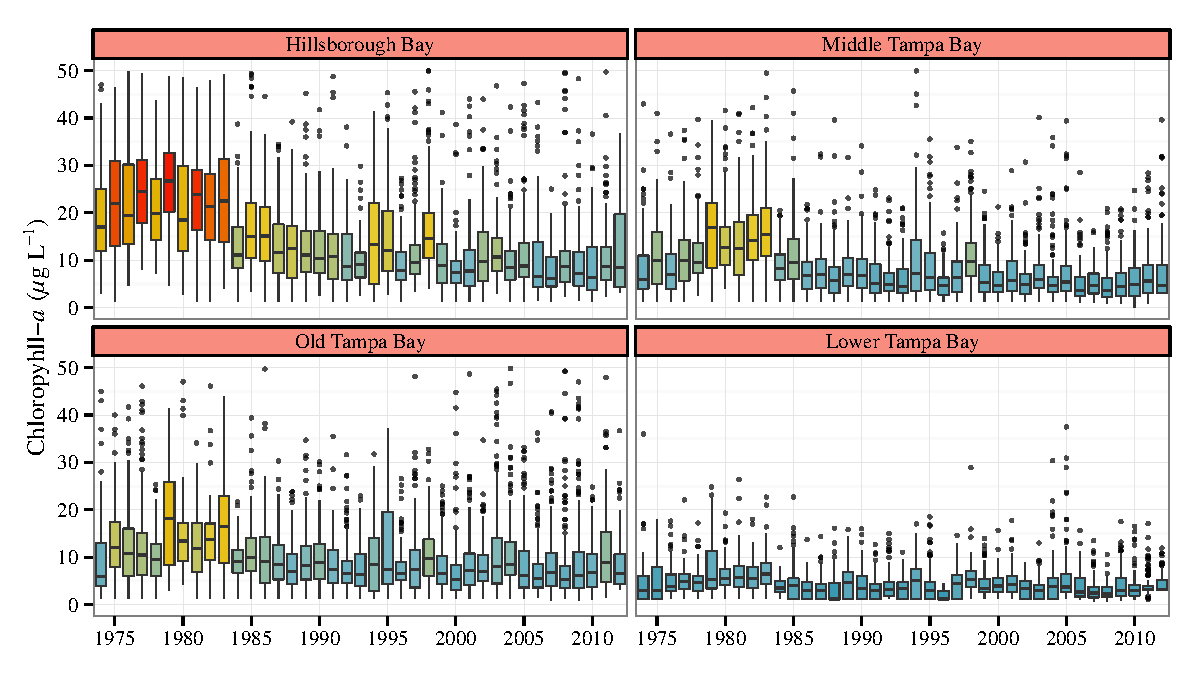
\includegraphics[width=\linewidth]{fig/annual_chl} 

}

\caption[Annual trends in chlorophyll for each bay segment]{Annual trends in chlorophyll for each bay segment.\label{fig:annual_chl}}
\end{figure}


\end{frame}

% variation in chl by year, season, and management

%%%%%%
\begin{frame}{\textbf{Tampa Bay}}{\textbf{Understanding chlorophyll response to eutrophication}}
What affects our interpretation of chlorophyll response to nutrients?
\vspace{-0.1in}
\captionsetup[subfloat]{captionskip=0pt, position=top}
\begin{figure}
\centering
\subfloat[]{
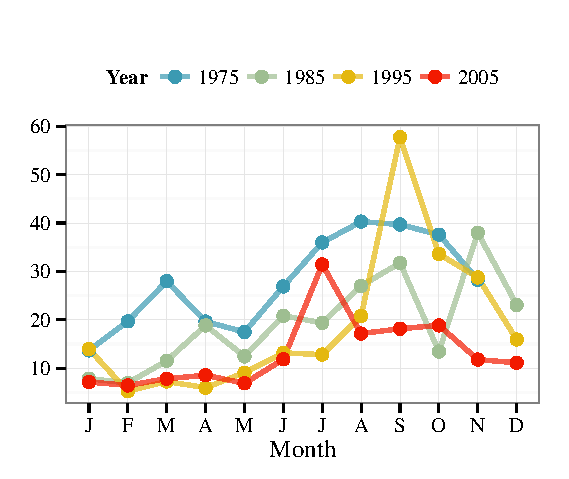
\includegraphics[width=0.46\textwidth,page=1,trim=0.2in 0in 0in 0.35in,clip]{fig/salmoyr.pdf}
\label{fig:salmoyr1}
}
\subfloat[]{
\includegraphics[width=0.46\textwidth,page=2,trim=0.2in 0in 0in 0.35in,clip]{fig/salmoyr.pdf}
\label{fig:salmoyr2}
}

\leavevmode\smash{\makebox[0pt]{\hspace{0em}% HORIZONTAL POSITION           
  \rotatebox[origin=l]{90}{\hspace{3em}% VERTICAL POSITION
    {\color{black} Chlorophyll-\textit{a}}}}}
    \hspace{0pt plus 1filll}\null

\caption{Variation in chlorophyll by {\color{zissou5}\protect\subref{fig:salmoyr1}} time and {\color{zissou5}\protect\subref{fig:salmoyr2}} salinity and management in Hillsborough Bay.  Panel {\color{zissou5}\protect\subref{fig:salmoyr1}} is colored before and after wastewater treatment in 1979.}
\label{fig:salmoyr}
\end{figure}
\captionsetup[subfloat]{position=top}
\end{frame}

%%%%%%
\begin{frame}{\textbf{Tampa Bay}}{\textbf{Understanding chlorophyll response to eutrophication}}
\alert{Problem:} Response endpoints of eutrophication vary naturally over time and with discharge or tidal patterns\\~\\
\alert{Solution:} Develop a model that accounts for changes in relationships between drivers of pollution over time.\\~\\
The \alert{weighted regression (WRTDS)} model is being developed by USGS for pollutant modelling in rivers \cite{Hirsch10}\\~\\
Models pollution concentration as a function of \alert{time}, \alert{discharge}, and \alert{season}\\~\\
\alert{Adaptation:} Can this approach be used to evaluate chlorophyll trends in Tampa Bay \cite{Beck15}?
\end{frame}



%%%%%%
\begin{frame}{\textbf{Tampa Bay}}{\textbf{Understanding chlorophyll response to eutrophication}}
How does weighted regression work?
\begin{center}
\animategraphics[controls,width=\linewidth]{12}{fig/wtex}{}{} %frame rate is 12 per/sec
\end{center}
\end{frame}

% prednrm figures


%%%%%%
\begin{frame}{\textbf{Weighted regression approach}}{\textbf{ Results for Tampa Bay}}
\only<1>{This gives us improved trend descriptions... \alert{observed predictions}}
\only<2>{This gives us improved trend descriptions... \alert{quantile predictions}}
\only<3>{This gives us improved trend descriptions... \alert{observed, flow-norm}}
\only<4>{This gives us improved trend descriptions... \alert{quantile, flow-norm}}
\includegraphics<1>[width=\textwidth,page=1]{fig/prednrm.pdf}
\includegraphics<2>[width=\textwidth,page=2]{fig/prednrm.pdf}
\includegraphics<3>[width=\textwidth,page=3]{fig/prednrm.pdf}
\includegraphics<4>[width=\textwidth,page=4]{fig/prednrm.pdf}
\end{frame}



%%%%%%
\begin{frame}{\textbf{Tampa Bay}}{\textbf{Understanding chlorophyll response to eutrophication}}
Because the model is dynamic, we have parameters describing the relationship of chlorophyll with other factors specific to different time periods \\~\\
\begin{columns}[T]
\begin{column}{0.45\textwidth}
\centerline{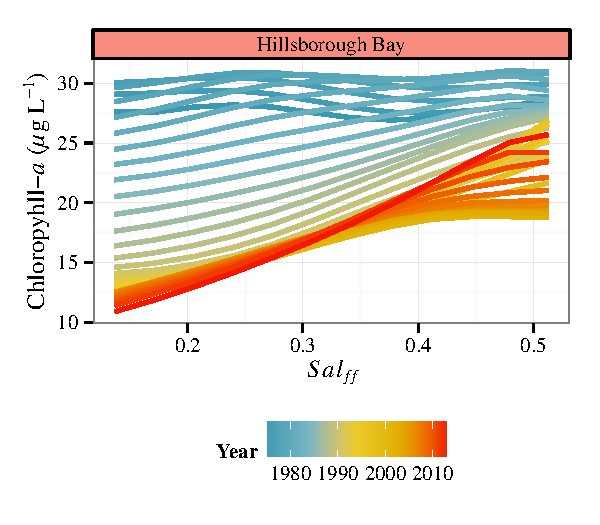
\includegraphics[width = \textwidth]{fig/hill.pdf}}
\end{column}
\begin{column}{0.45\textwidth}
\begin{itemize}
\item Early period (blue) - point-sources
\item Late period (red) - non-point sources
\item Chlorophyll shows increasing response to freshwater input in recent years
\end{itemize}
\end{column}
\end{columns}
\end{frame}

%%%%%%
\begin{frame}{\textbf{Tampa Bay}}{\textbf{Understanding chlorophyll response to eutrophication}}
What does this mean for Tampa Bay and elsewhere?\\~\\
\begin{itemize}
\item Predictions followed observed chlorophyll -- but increased clarity in the description
\item More detailed evaluation of trends allows greater insight into drivers of change\\~\\
\end{itemize}
The model parameters show us a picture...
\centerline{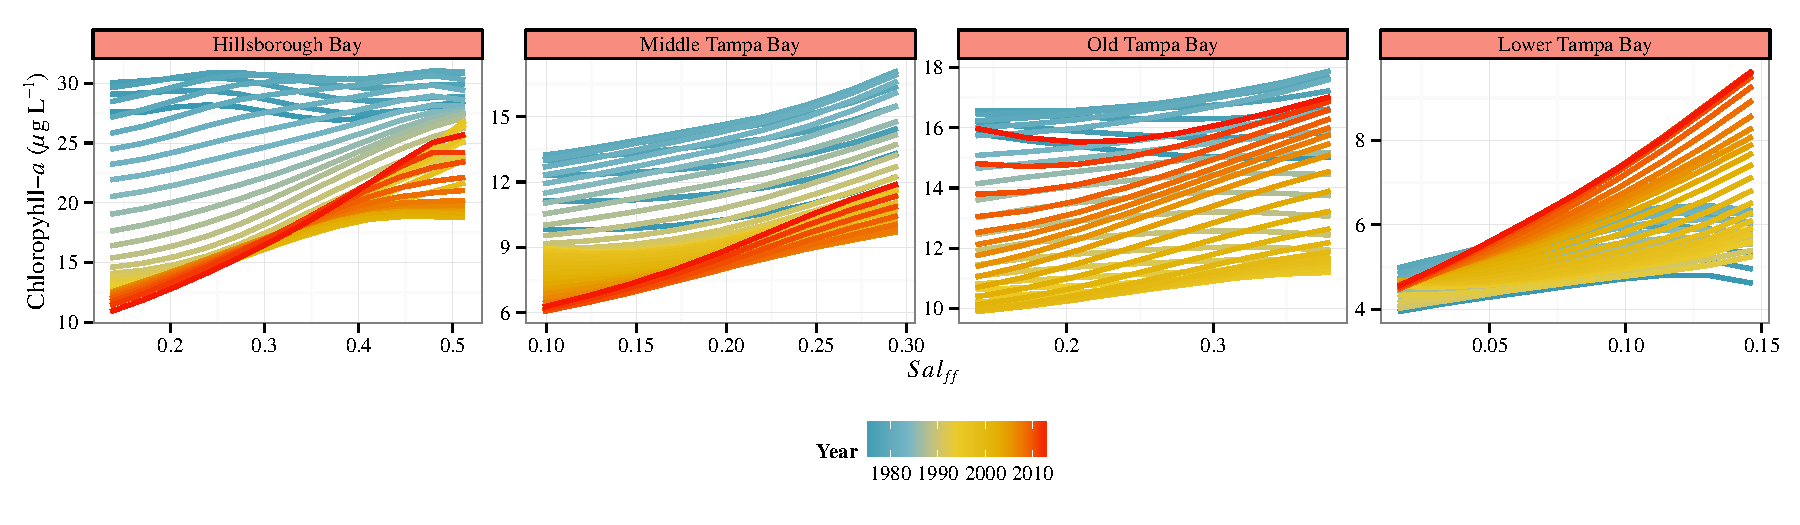
\includegraphics[width = \textwidth]{fig/title_plo.pdf}}
\end{frame}

% patux map


% patux trends


%%%%%%
\begin{frame}{\textbf{WRTDS adaptations and products}}{\textbf{ Additional study systems}}
Currently comparing WRTDS and GAMs for trend evaluation
\begin{columns}
\begin{column}{0.38\textwidth}
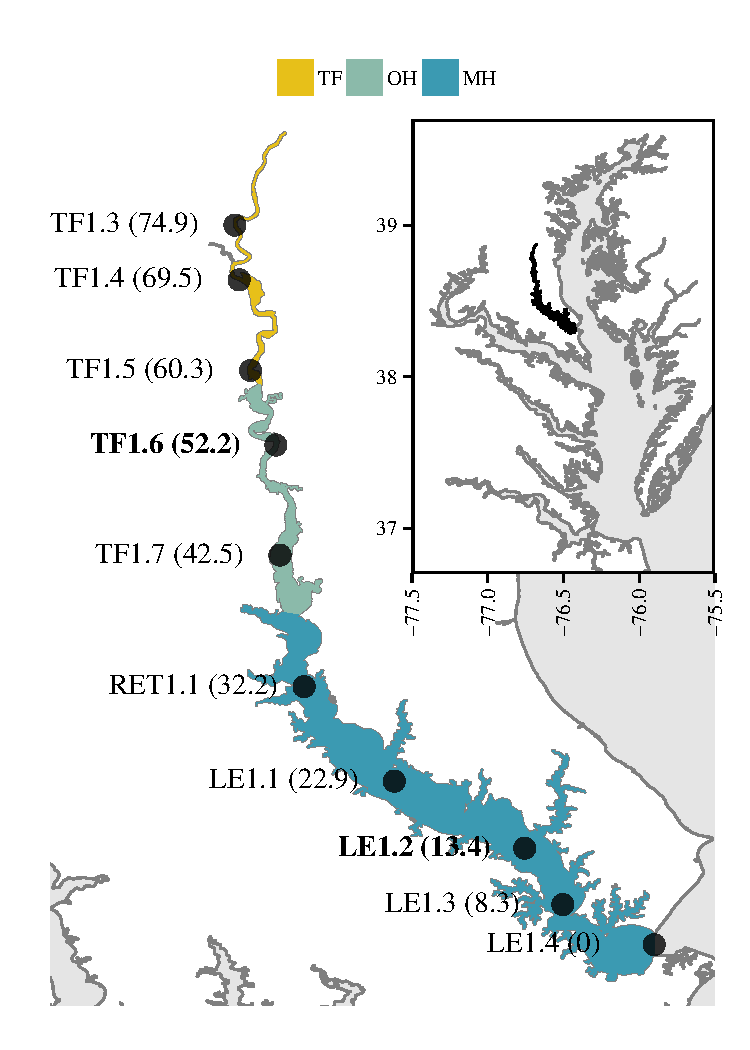
\includegraphics[width = \textwidth]{fig/patux_map.pdf}
\end{column}
\begin{column}{0.65\textwidth}
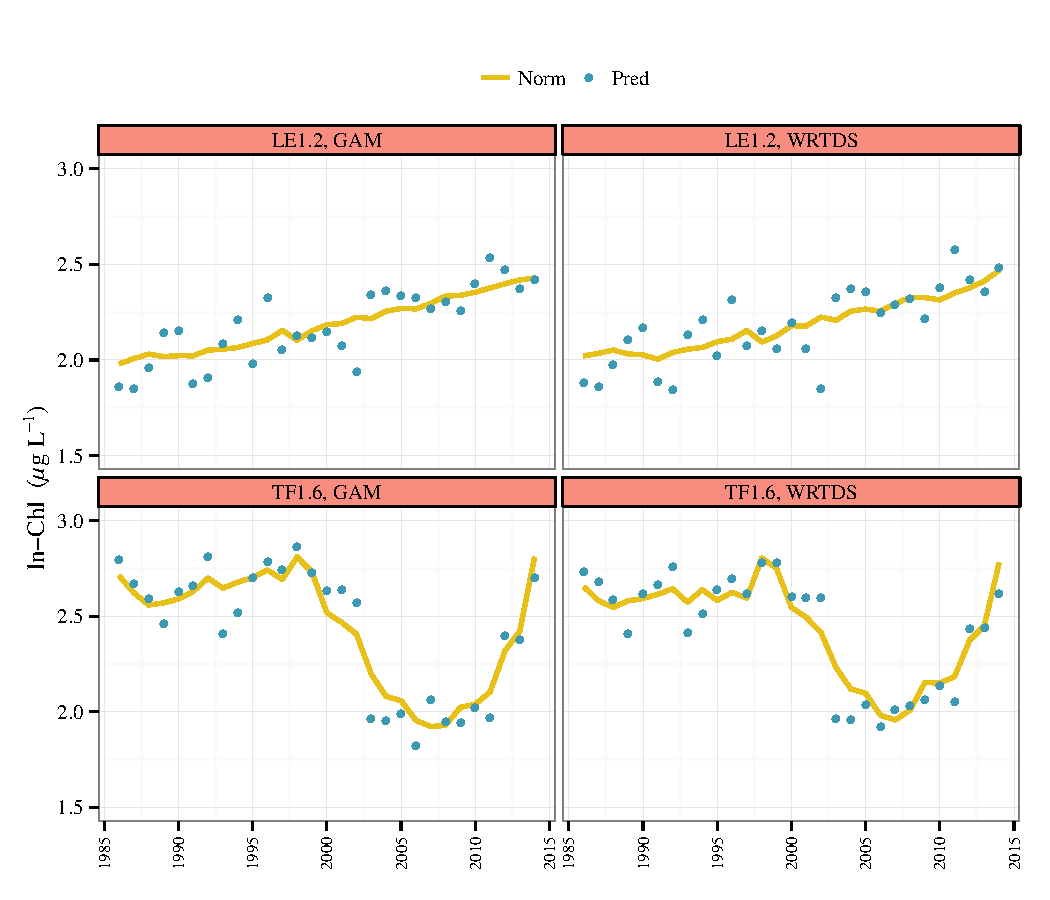
\includegraphics[width = \textwidth]{fig/predann.pdf}
\end{column}
\end{columns}
\end{frame}

%%%%%%
\begin{frame}{\textbf{WRTDS adaptations and products}}{\textbf{ Additional study systems}}
Adapting weighted regression to `detide' dissolved oxygen time series \cite{Beck15b}\\~\\

\includegraphics[width = \textwidth]{fig/lopaper.png} \\~\\
\centerline{\alert{Wednesday 11:15, B110-112}}
\end{frame}

%%%%%%
\begin{frame}
\alert{Acknowledgments:}\\~\\
\begin{columns}
\begin{column}{0.6\textwidth}
{\footnotesize
Research staff and employees at USEPA Gulf Ecology Division \\~\\
Field staff and data managers at Hillsborough County Environmental Protection Commission\\~\\
Research coordinators, technicians, and field staff of the National Estuarine Research Reserve System}\\~\\
\end{column}
\begin{column}{0.3\textwidth}
\vspace{-0.2in}
\begin{center}
{\tiny
Wes Anderson Zissou color theme borrowed and adapted from \href{https://github.com/karthik/wesanderson}{github.com/karthik}\\~\\
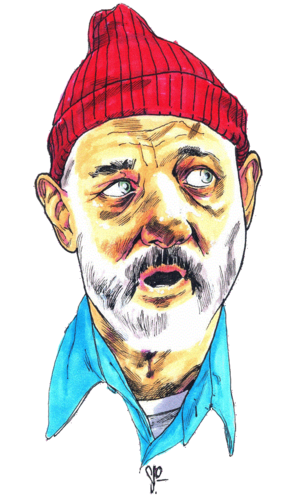
\includegraphics[width=0.55\linewidth]{fig/zissou.png}\\~\\
\vspace{-0.15in}
\scalebox{0.7}{\hbox{\tiny Image credit:\thinspace{\tiny \href{http://stephenmorrow.deviantart.com/}{Stephen Morrow}}}}}
\end{center}
\end{column}
\end{columns}
\vfill
\alert{Funding sources and contact:}\\~\\
\begin{columns}
\begin{column}{0.4\textwidth}
\centerline{
\includegraphics[width=0.5\linewidth]{fig/epa_logo.png}}
\end{column}
\begin{column}{0.6\textwidth}
\scriptsize
\href{mailto:beck.marcus@epa.gov}{beck.marcus@epa.gov} \\~\\
Phone: 8509342480 \\~\\
Blog: \href{http://beckmw.wordpress.com/}{http://beckmw.wordpress.com/} \\~\\
\alert{WRTDS tidal package:} \href{https://github.com/fawda123/wtreg_for_estuaries}{https://github.com/fawda123/wtreg\_for\_estuaries}
\end{column}
\end{columns}
\vspace{0.2in}
\end{frame}

%%%%%%
\begin{frame}[t]{\textbf{References}}
\tiny
\setbeamertemplate{bibliography item}{}
\bibliographystyle{apalike_mine}
\bibliography{ref_diss}
\end{frame}

\end{document}
